% Systematisk beskrivelse af konfigurations tabel.
\section{Konfigurationstabel}
En konfiguration af et system er en kombination af elementer, og en konfigurationstabel beskriver den konfiguration.

Denne beskrivelse er baseret på \citet[Afsnit 3.2, Side 16-21]{art:essence}.

Den øverste række i \cref{tab:konfigurationsTabel} navngiver de fire Views i Essence: Paradigm, Product, Project og Process.

`Focus' rækken repræsenterer de største problemer og løsninger i projektet. 
Udfordringen er tiltænkt til at være om man kan bruge en mobil til at overvåge adfærd af unipolare og bipolare patienter og gøre dem opmærksom på adfærdsændringer og dette er så tiltænkt at disse patienter åbner en applikation på denne mobil hvor de vil blive blive givet et overblik og derved få at vide om der har været adfærdsændringer. 
Det er så vigtigt at systemet skal kun observere og informere.
Løsnings strategien er så at bruge en smartphone, og udvikle et system som kan registrere data fra forskellige sensor moduler og gemme det på telefonen som den bliver brugt af patienten.
Data den indsamler skal være objektiv og spore patientens sindstilstand såsom en fitness tracker sporer fysisk tilstand samt at systemet skal være ekspandérbart, så vision for systemet er så at den skal fungere som en fitness tracker, en objektiv dagbog og et F-16 fly.
Denne data kan så bruges til analyse og blive undersøgt om der er nogle ændringer i patientens opførsel og skal let kunne aflæses af patienten hvorfra de kan få relevant information fra den præsenterede data. 

`Overview' rækken repræsenterer projektets stakeholders. Hoved perspektivet er selvfølgelig fra patienterne, da det er dem som skal bruge produktet men der er også sponsorer som er interesseret i at se projektet være en succes da det vil gøre at deres patienter vil få det nemmere. 
Designet på projektet er simpelt idet der bruges mobil eller wearables til sensor input og at denne data gemmes og analyseres på mobilen, og at det skal udvikles på Android.
Argumentet for at lave et sådant projekt er, at depression og mani ofte opdages for sent, hvilket i det fleste tilfælde gør situationen værre.
Hvis symptomerne identificeres så perioden opdages tidligt kan den måske forhindres, hvilket kan spare staten en del udgifter til behandlinger og indlæggelser.
Der er dog det problem at en smartphone baseret løsning som der her sigtes efter selvfølgelig kræver en smartphone, og også stiller lidt krav til at folk kan bruge deres smartphone.
Dette er dog bare et minimalt problem da en stor del at befolkningen har smartphone nu om dage så derfor kan man også gå ud fra de kan finde ud af at bruge den på et acceptabelt niveau.
Selv hvis en potentiel bruger ikke har en smartphone, koster den lettilgængelige teknologi ikke så meget, så at investere i den som et behandlingsmiddel er en reel mulighed.
For at evaluere systemet kan der bruges et fokusgruppemøde og integrationstest for at sikre det er modulær, fleksibel, kombinerbar og kommunikativ.

`Details' rækken repræsenterer nøgle scenarier, nøgle komponenter og features.
Desuden indeholder det sidste felt i denne række også findings.
Findings er speciel da den bruges som et input til den næste Sprint Planning aktivitet, se \citet[Afsnit 8.5, Side 54]{art:essence}. 
Findings kommer som et resultat af evaluering af systemet. 
Disse findings er at der er problemer med højt pladsforbrug og at systemet har mulige sikkerhedsproblemer. 

\begin{figure}
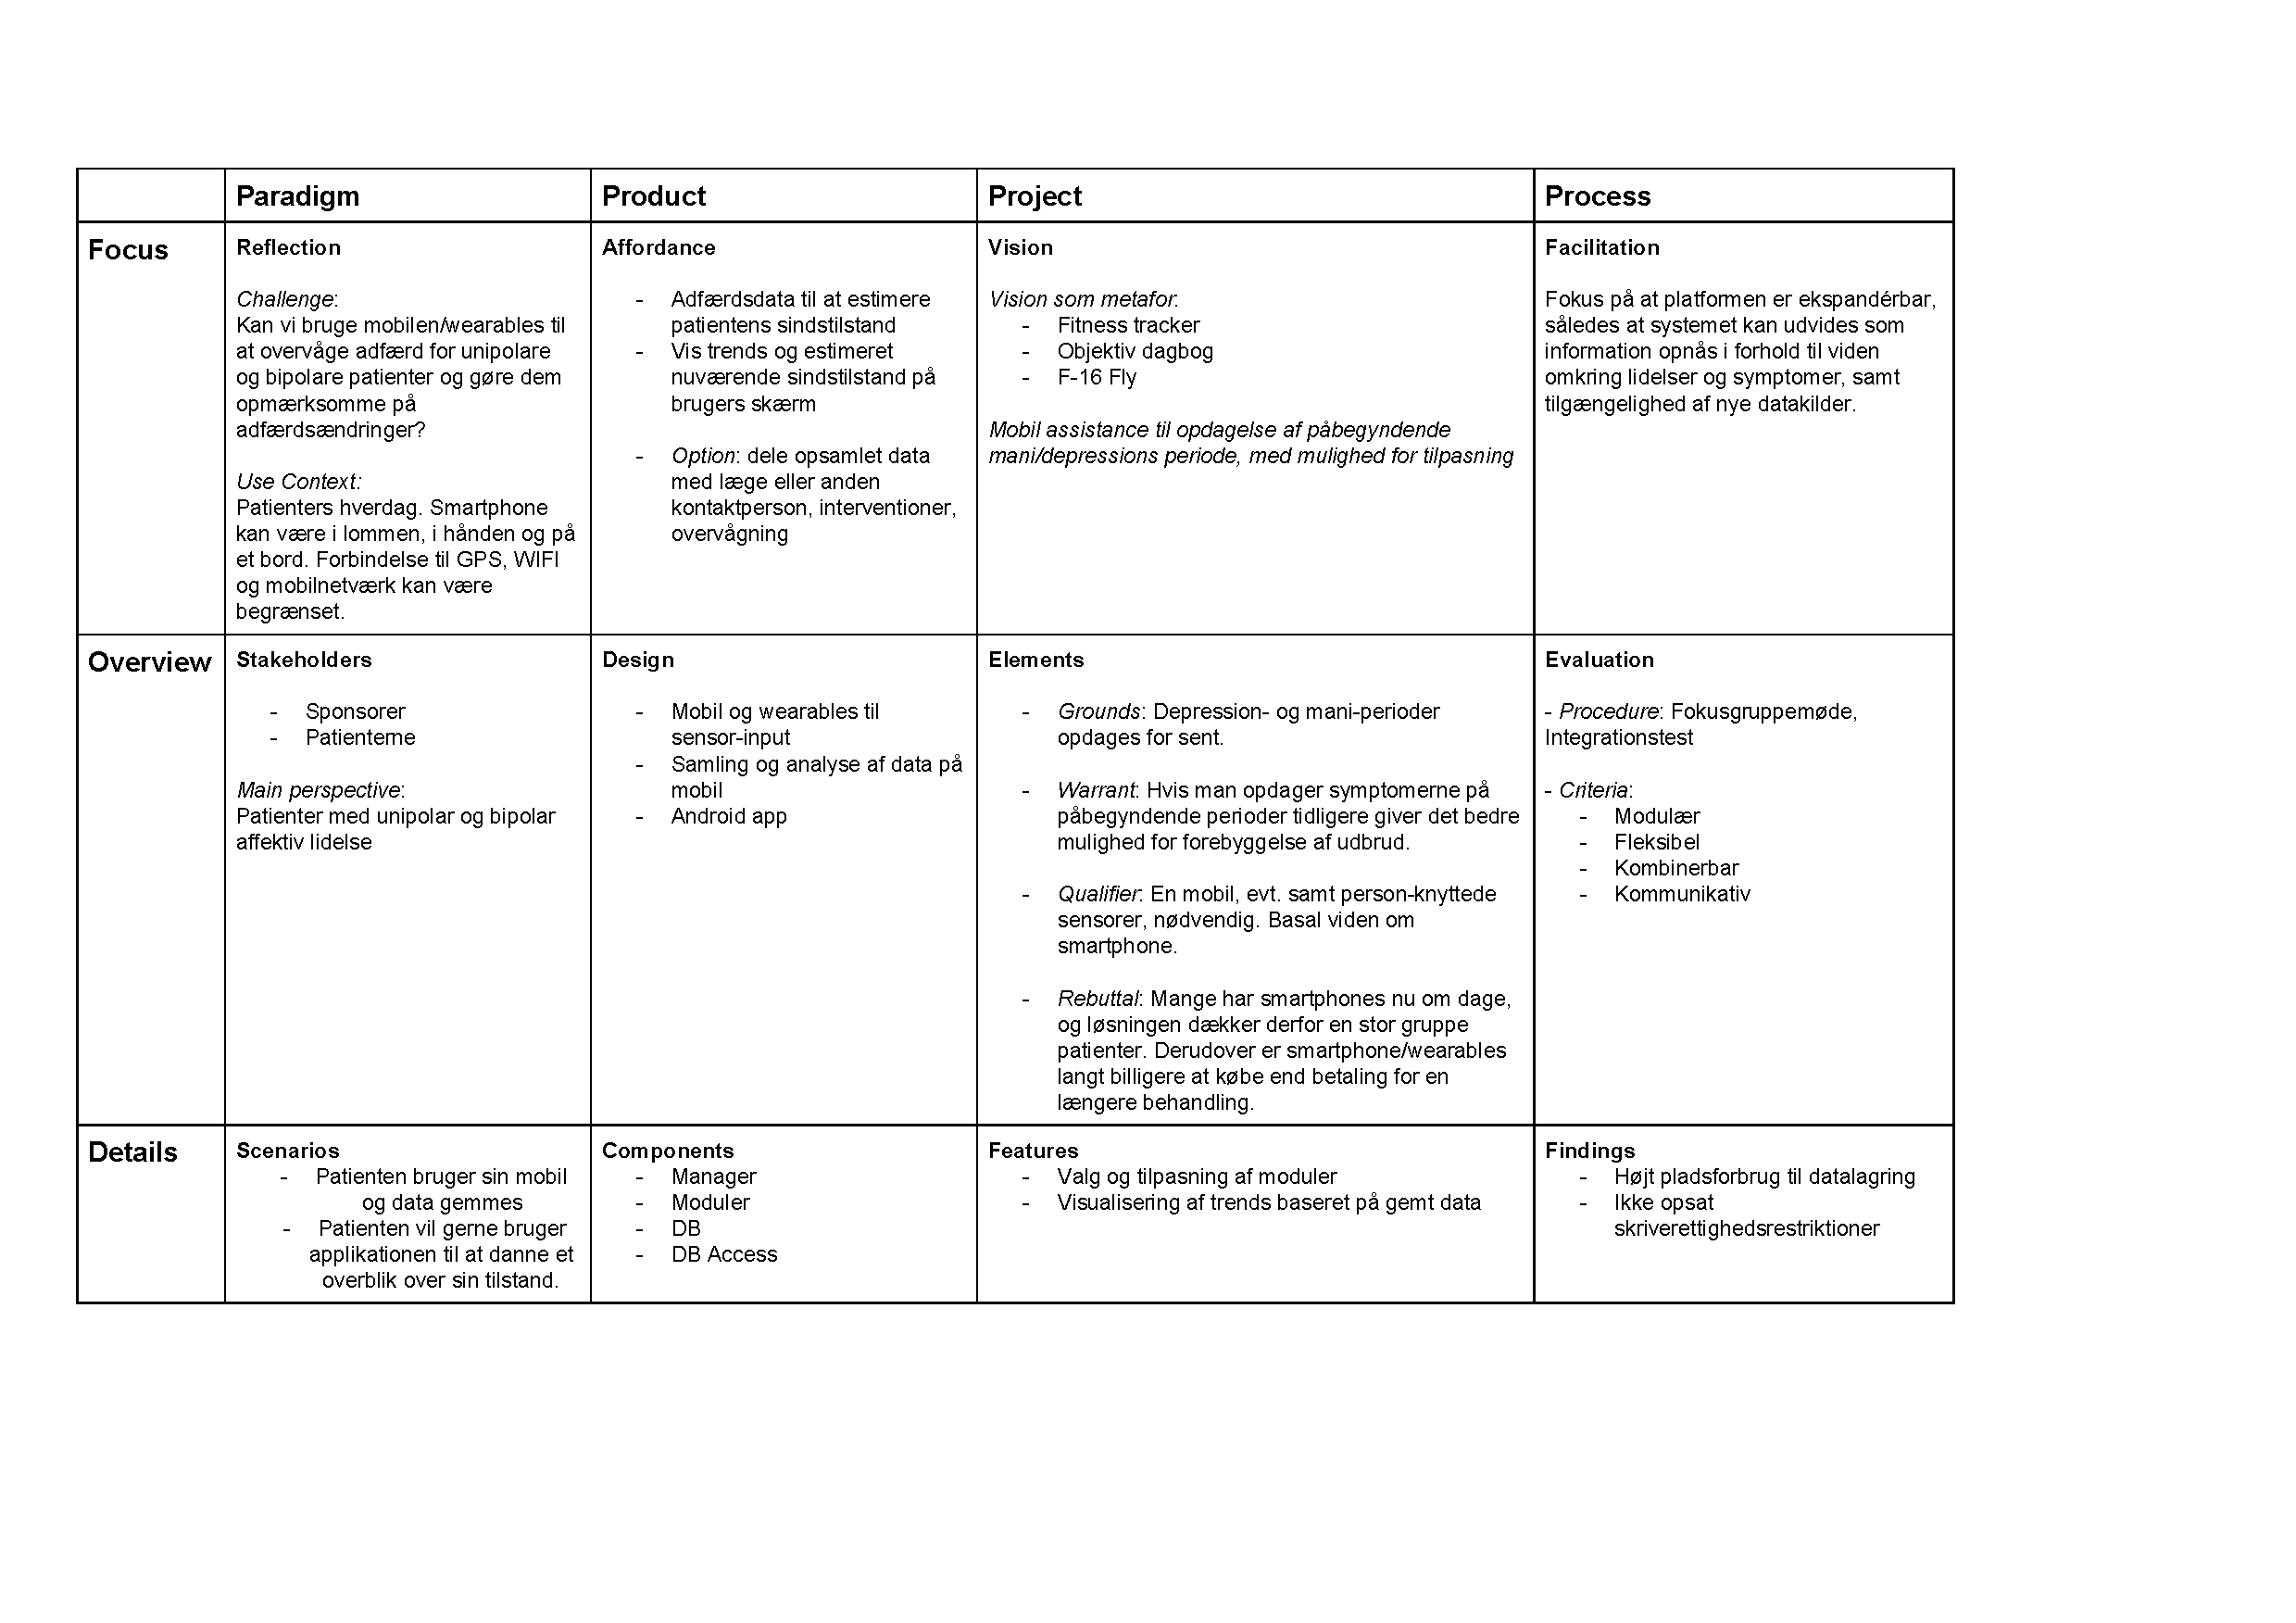
\includegraphics[scale = 0.65,trim = 1cm 3cm 6cm 2cm, angle = 90, clip]{KonfigurationTabel-frarapport.pdf}
\caption{En konfigurationstabel af systemet.}
\label{tab:konfigurationsTabel}
\end{figure}
